\documentclass[10pt,a4paper]{article}
\usepackage[utf8]{inputenc}
\usepackage[russian]{babel}
\usepackage[OT1]{fontenc}
\usepackage{amsmath}
\usepackage{amsfonts}
\usepackage{amssymb}
\usepackage{makeidx}
\usepackage{graphicx}

\usepackage{graphicx}
\usepackage{caption}
\usepackage{subcaption}

\usepackage{float}
\floatstyle{boxed}
\restylefloat{figure}

\author{Максим Борисяк}
\title{Дипломная работа}
\makeindex

\newtheorem{defen}{Определение}

\newcommand{\stock}{\text{STOCK}}
\newcommand{\source}{\text{SOURCE}}

\textheight = 720pt
\textwidth = 500pt

\hoffset = -25mm
\voffset = -30mm

\begin{document}

\maketitle

\section{Введение}

Введение.

\subsection{Мотивация}
Мотивация

\subsection{Базовые понятия и определения}
В данном разделе будут введены базовые понятия, используемые в данной работе, в том числе,
понятия атомарного блока, составного блока, потока данных, автомата Мили соответствующего блоку и так далее.

Основной единицей потока данных является так называемый атомарный блок.
\begin{defen}
  \textbf{Атомарным блоком} $b$ назовем некий элемент имеющий два непересекающихся набора портов: \textit{входной} и \textit{выходной}.
  Введем так же функции $inputs(b)$ и $outputs(b)$ равные множетвам входных и выходных портов блока $b$ соответственно.
\end{defen}

В реальных системах для построения и запуска потока данных атомарный блок представляется в виде подпрограммы или модуля
(функции, класса некого объектно ориентированного языка программирования, динамической библиотеки), который используя данные некого набора своих входных портов, вычисляет
и записывает данные в свои выходные порты.
В такой интерпретации некую вычислимую функцию $f(x_1, x_2, \dots, x_n)$ можно представить в виде блока $b_f$
с входными портами $x_1, x_2, \dots, x_n$ и одним выходным портом $F$, который при получении данных со всех входных портов
выписывает значения функции $f(x_1, x_2, \dots, x_n)$ в порт $F$.

Как правило, конкретный блок является копией некого шаблона или экземпляром некого класса (по аналогии с понятием экземпляра класса в ОО языках программирования).

На рисунке \ref{map} схематично изображен блок класса \textit{Map}, для которого $inputs(Map) = \{xs, f\}$, $outputs(Map) = \{fs, x\}$.

\begin{figure}[H]
  \centering

  \begin{subfigure}[b]{0.2\textwidth}
    \centering
    \label{map:connection}
    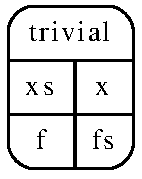
\includegraphics[width=\textwidth]{map_cg.pdf}
    \caption{Схема блока}
  \end{subfigure}
  ~
  \begin{subfigure}[b]{0.7\textwidth}
    \centering
    \label{map:fa}
    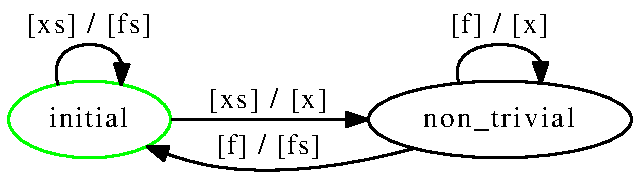
\includegraphics[width=\textwidth]{map_fa.pdf}
    \caption{Автомат Мили блока}
  \end{subfigure}
  
  \label{map}
  \caption{Схематичное изображение блока класса \textit{Map} (a) и соответствующего ему конечного автомата Мили (b).}
\end{figure}

Основной структурой для построения схемы потока данных является составной блок.

\begin{defen}
 \textbf{Составным блоком} будем называть кортеж $c = (B, E, I, O)$, где:
 \begin{itemize}
    \item $B$ - множество блоков;
    \item $E$ - множество ребер вида $e_b = (b_1, b^O_{1}, b_2, b^I_{2})$, $b_1, b_2 \in B$, $b^O_{1} \in outputs(b_1), b^I_{2} \in inputs(b)$,
                либо вида $e_I = (c^I, b, b^I)$, $e_O = (b, b^O, c^O)$, где $b \in B$, $b^I \in inputs(b)$, $b^O \in outputs(b)$, $c^O \in O$, $c^I \in I$.
                Множества ребер $e_b$ будем обозначать как $E^B$, $e_I$ и $e_O$ как $E^I$ и $E^O$ соответственно.
    \item $I$, $O$ - наборы входных и выходных портов (по аналогии с атомарным блоком).
  \end{itemize}
  Аналогично атомарному блоку определяются функции $inputs(c) = I$ и $outputs(c) = O$.
\end{defen}

Иногда удобно рассматривать иное представление составного блока, добавляя фиктивные блоки $\stock$, $inputs(\stock) = O$, $outputs(\stock) = \varnothing$
  и $\source$, $inputs(\source) = \varnothing$, $outputs(\source) = I$:
$$\hat{E}^I = \{(\source, \source^O, b, b^I) \vert (\source^O, b, b^I) \in E^I\}$$
$$\hat{E}^O = \{ (b, b^O, \stock, \stock^I) \vert (b, b^O, \stock) \in E^O \}$$
$$\hat{B} = (B \cup \{\stock, \source\}, E^B \cup \hat{E}^I \cup \hat{E}^O)$$

В этом случае составной блок $\hat{B}$ описывается графом с ребрами вида $(u, u^O, v, v^I)$. На рисунке \ref{example} изображен пример составного блока.

\begin{figure}[H]
  \centering
  
  \begin{subfigure}[b]{0.3\textwidth}
    \centering
    \label{example:composite}
    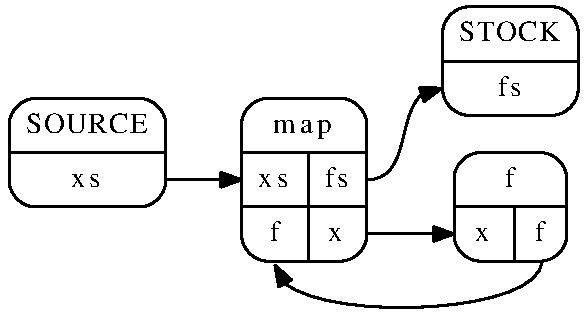
\includegraphics[width=\textwidth]{example_cg.pdf}
    \caption{Составной блок}
  \end{subfigure}
  ~
  \begin{subfigure}[b]{1.0\textwidth}
    \centering
    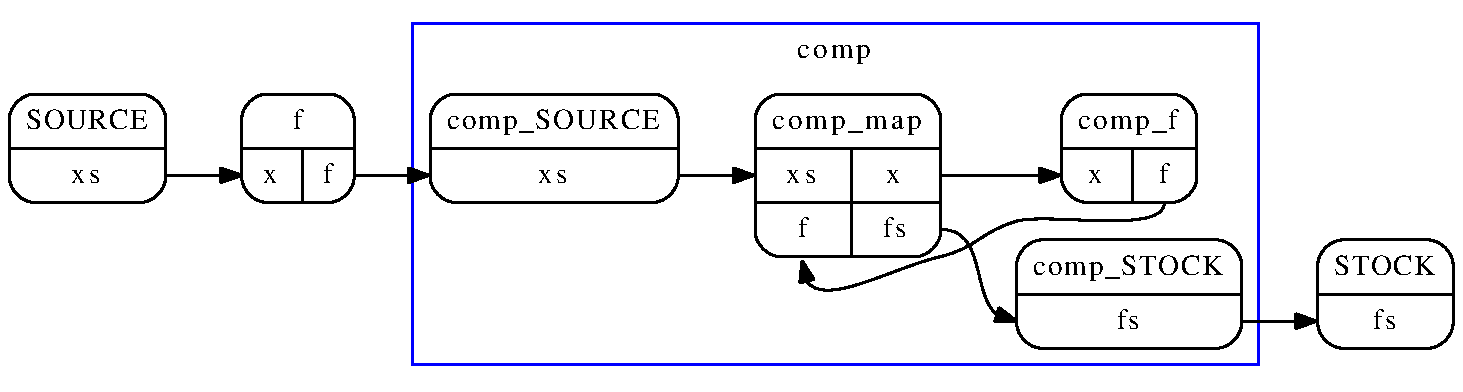
\includegraphics[width=\textwidth]{cc_cg.pdf}
    \label{example:supercomposite}
    \caption{Супер-составной блок}
  \end{subfigure}
  
  \caption{ Примеры графов составного и супер-составного блока.}
  \label{example}
\end{figure}

\end{document}